% =====================================================================
%  週次進捗報告 2026/09/23 — 雛形（骨組みのみ）
%
%  この .tex は Claude Code が「枠」だけ作ったものです。
%  ・見出し、図表の枠、数値の表 …… 入っています（数値は実測・実計算値）
%  ・本文（\par 以下の説明文） ……… 空けてあります。% TODO(Antigravity) の
%    箇所を埋めてください。材料は HANDOFF.md の 2026-09-23 エントリにあります。
%
%  ビルド:  .\build_report.ps1 20260923_report
%  文字コード: UTF-8 (BOM なし) / pTeX (ptex2pdf)、pdflatex ではない
% =====================================================================
\documentclass{jarticle}
\usepackage[dvipdfmx]{graphicx}
\topmargin       -10.0mm
\oddsidemargin   -0.4mm
\evensidemargin  -0.4mm
\headheight       0.0mm
\headsep          0.0mm
\footskip        10.0mm
%
\textheight     260.0mm
\textwidth      170.0mm
%
\setlength{\parindent}{1zw}
%
\usepackage{graphicx}
\usepackage{multirow}
\usepackage{wrapfig}
\makeatletter
\def \fgcaption{\def \@captype{figure} \caption}
\def \tbcaption{\def \@captype{table} \caption}
\makeatother
\def \figurename{Fig.}
\def \tablename{Table}
%
\def\topfraction{.99}
\def\bottomfraction{.99}
\def\textfraction{.01}
\def\floatpagefraction{.99}
%
\pagestyle{empty}
%
\begin{document}
%
\begin{center}
 \begin{tabular}{|c|c|c|} \hline
  \parbox{50mm}{\vspace{1mm} \centering{\Large\bf 2026/09/23}} &
  \parbox{55mm}{\vspace{1mm} \centering{\Large\bf B4　堀田裕樹}} &
  \parbox{50mm}{\vspace{1mm} \centering{\Large\bf No.~13}}
  \\ [2mm] \hline
%
  \multicolumn{3}{|c|}{%
   \parbox{155mm}{\centering\Large\bf
    \vspace{1mm}
    音響ウッド異常における二重モード変換の機構と本研究条件への適用
   }
  }
  \\ [2mm] \hline\hline
%
  \multicolumn{3}{|c|}{%
   \parbox{155mm}{\large\vspace{1mm}
%
    {\Large\bf 今週の進捗要点}
%
    \begin{itemize}
     \item Liu らの2編（2017年論文・2018年博士論文）の精読と，音響ウッド異常の物理機構の整理
     \item 二重モード変換が表面共振の再放射方向を界面法線に決めることの確認
     \item 回折格子方程式 $f = mc/\Lambda$ を本研究の鋼／空気系に適用した異常周波数の算出
     \item 実験平均波形のメインバン・テイル分離解析による予備的検証
    \end{itemize}
%
   }
  }
  \\ [2mm] \hline
 \end{tabular}
\end{center}

\par
今週は，周期凹凸と超音波の相互作用について論じた Liu らの文献2編を精読し，本研究の実験条件に当てはめて何が言えるか（特に音響ウッド異常と二重モード変換の観点から）を検討した．さらに，実験の平均波形を用いてメインバンとテイルの分離解析を行い，予備的な検証を実施した．


% =====================================================================
\section{読んだ論文}
% =====================================================================
\begin{description}
 \item[{[1]}] J.~F.~Liu and N.~F.~Declercq,
   ``Acoustic Wood anomaly in transmitted diffraction field,''
   {\it AIP Advances} {\bf 7}, 035116 (2017).
 \item[{[2]}] J.~Liu,
   ``Interaction of ultrasound with periodic and composite structures,''
   Ph.D. thesis, Universit\'e de Lorraine (2018).
\end{description}

\par
これらの文献は，周期的な凹凸界面に超音波が垂直入射した際の散乱・回折現象（音響ウッド異常）や，それに伴うモード変換について詳細に解析している．本研究で対象としている鋼板中の鋸歯状・矩形溝も「周期的な溝からの反射」という同一の問題設定に帰着できるため，現象の物理的解釈や超音波評価の可能性を探る上で極めて重要な示唆を与える．


% =====================================================================
\section{音響ウッド異常の物理機構}
% =====================================================================

\subsection{異常周波数を決める条件（モード変換仮説）}
\par
周期 $\Lambda$ の凹凸界面に広帯域の超音波が垂直入射したとき，特定の周波数において入射バルク波が界面上の表面型波（エバネッセントモード）へとモード変換される．この現象が「音響ウッド異常」の生じる条件であり，その周波数は古典的回折格子方程式から導かれる．
垂直入射（$\theta^i = 0$）のとき，古典的回折格子方程式は
\begin{equation}
 \sin\theta_m^d = m\,\frac{\lambda^d}{\Lambda}
\end{equation}
となる．ある回折次数が界面に沿って生成される条件 $\theta_m^d = 90^\circ$ を課すと，
変換された波の速度は
\begin{equation}
 c^d = \frac{f\,\Lambda}{m}
 \label{eq:grating}
\end{equation}
で与えられる（$\Lambda$：凹凸周期，$m$：回折次数）．

\par
式(\ref{eq:grating}) で求めた $c^d$ を媒質固有の波の速度と突き合わせ，最も近いものをモード変換後の波種とみなす（速度整合法）ことで，どのモードが励起されたかを判定できる．なお，文献[2]（表2-2，2.3.4.2節）によれば，固体-流体界面とは異なり，固体-空気（真空）界面において生成される表面波はレイリー波のみである．


\subsection{二重モード変換}
\par
前節の条件を満たすとき，入射バルク波は界面上の表面型波へと変換される（第1のモード変換）．生成された表面型波は凹凸界面に沿って伝搬する過程で強く減衰し，表面振動として凹凸構造と結合して表面共振を励起する．続いて，この表面共振が凹凸によって再び回折され，バルク波へと逆変換される（第2のモード変換）．

この第2のモード変換において，入射波（表面共振）は界面に平行に進むため $\sin\theta^{i,II} = 1$ であり，
回折格子方程式は
\begin{equation}
 \frac{1}{\lambda^{i,II}} + \frac{\sin\theta_m^{d,II}}{\lambda^{d,II}} = \frac{m}{\Lambda}
\end{equation}
となる．$\lambda^{i,II} = \lambda^{d,I}$，$\lambda^{d,II} = \lambda^{i,I}$ を用いると
\begin{equation}
 \sin\theta_m^{d,II}
  = \lambda^{i,I}\left(\frac{m}{\Lambda} - \frac{1}{\lambda^{d,I}}\right) = 0
 \label{eq:double}
\end{equation}
すなわち $\theta^{d,II} = 0^\circ$ が得られる．


\subsection{ディップ・ティップは FFT が作る仮想的な干渉である}
\par
文献[2]によれば，受信波形は直達反射である「メインバン」と，遅れて到達する「テイル（後続振動）」に時間的に分離している．異常周波数におけるスペクトルの構造（ディップやティップ）を作り出している原因はこのテイルであり，メインバンのみを窓処理で切り出すと異常は消失する．

したがって，観測されるディップは物理的な破壊的干渉によってエネルギーが失われた結果ではなく，時間的に分離したメインバンとテイルの2成分を FFT が複素加算したことによって生じる「仮想的な干渉」の産物にすぎない．両者の位相差が $\pi/2$ より大きければ打ち消し合ってディップとなり，$\pi/2$ より小さければ強め合ってティップとなる．実際，ソノグラム（時間-周波数表示）を用いた解析により，異常周波数のエネルギーは失われているのではなく，単に遅れて到達しているだけであることが確認されており，従来の「エネルギー損失仮説」は明確に否定されている．この知見は，本研究における窓処理（テイルを切り落とすか否か）の妥当性を検討する上で極めて重要である．


% =====================================================================
\section{本研究の条件への適用}
% =====================================================================
\par
前述の物理機構を，本研究で用いている鋼と探触子の条件に適用し，異常周波数の予測を行った．
本研究の鋼（$\rho = 7840\,\mathrm{kg/m^3}$, $E = 206\,\mathrm{GPa}$,
$G = 80\,\mathrm{GPa}$, $\nu = 0.27$）では
$c_l = 5730\,\mathrm{m/s}$, $c_t = 3194\,\mathrm{m/s}$,
$c_R = 2942\,\mathrm{m/s}$ である．探触子の中心周波数は $f_0 = 4.7\,\mathrm{MHz}$
（$\lambda_P = 1.219\,\mathrm{mm}$, $\lambda_S = 0.680\,\mathrm{mm}$,
$\lambda_R = 0.626\,\mathrm{mm}$）．
底面は鋼と空気の界面であるため，生成されうる表面波はレイリー波のみである．

\begin{center}
 \tbcaption{式(\ref{eq:grating}) による異常周波数の予測値 [MHz]．
  $\ast$ は探触子の帯域内に入るもの．}
 \vspace{1mm}
 \begin{tabular}{|c|c|r|r|r|r|} \hline
  $\Lambda$ [mm] & モード & $m=1$ & $m=2$ & $m=3$ & $m=4$ \\ \hline\hline
  \multirow{3}{*}{1.25}
   & Rayleigh & $2.354^\ast$ & $4.708^\ast$ & $7.062^\ast$ & 9.416 \\
   & S        & $2.556^\ast$ & $5.111^\ast$ & $7.667^\ast$ & 10.222 \\
   & P        & $4.584^\ast$ & 9.168        & 13.752       & 18.336 \\ \hline
  \multirow{3}{*}{2.00}
   & Rayleigh & $1.471^\ast$ & $2.942^\ast$ & $4.414^\ast$ & $5.885^\ast$ \\
   & S        & $1.597^\ast$ & $3.194^\ast$ & $4.792^\ast$ & $6.389^\ast$ \\
   & P        & $2.865^\ast$ & $5.730^\ast$ & $8.595^\ast$ & 11.460 \\ \hline
 \end{tabular}
 \label{tab:predicted}
\end{center}

\par
表\ref{tab:predicted} に示すように，$\Lambda = 1.25\,\mathrm{mm}$ の場合，レイリー波の $m=2$ モードの異常周波数が 4.708 MHz となり，探触子の中心周波数 4.7 MHz とわずか 0.2\% の差で一致している．さらに，文献[2]の実験試料（$H/\Lambda \approx 0.135$, $\Lambda/\lambda \approx 1\sim1.4$）と本研究の形状比を比較すると，$H/\Lambda$ は 0.10（$\Lambda=2.00\,\mathrm{mm}$）および 0.16（$\Lambda=1.25\,\mathrm{mm}$），$\Lambda/\lambda$ は $\Lambda=2.00\,\mathrm{mm}$ において P波で 1.64，S波で 2.94 と同オーダーである．したがって，本研究の測定条件は回折が十分に効く領域に入っており，実データにおいても音響ウッド異常が顕著に現れる可能性が高いと言える．


% =====================================================================
\section{実験波形による予備的検証}
% =====================================================================
\par
前節の予測を踏まえ，実験の平均波形（全18条件）を用いて予備的な検証を行った．解析対象の波形を，包絡線のピーク位置を基準として「メインバン（ピーク $-0.15 \sim +0.30\,\mathrm{\mu s}$）」と「テイル（ピーク $+0.6\,\mathrm{\mu s}$ 以降）」に時間領域で分離し，それぞれ独立に FFT を適用してスペクトルを比較した．

\begin{center}
  \begin{minipage}[b]{0.49\linewidth}
    \centering
    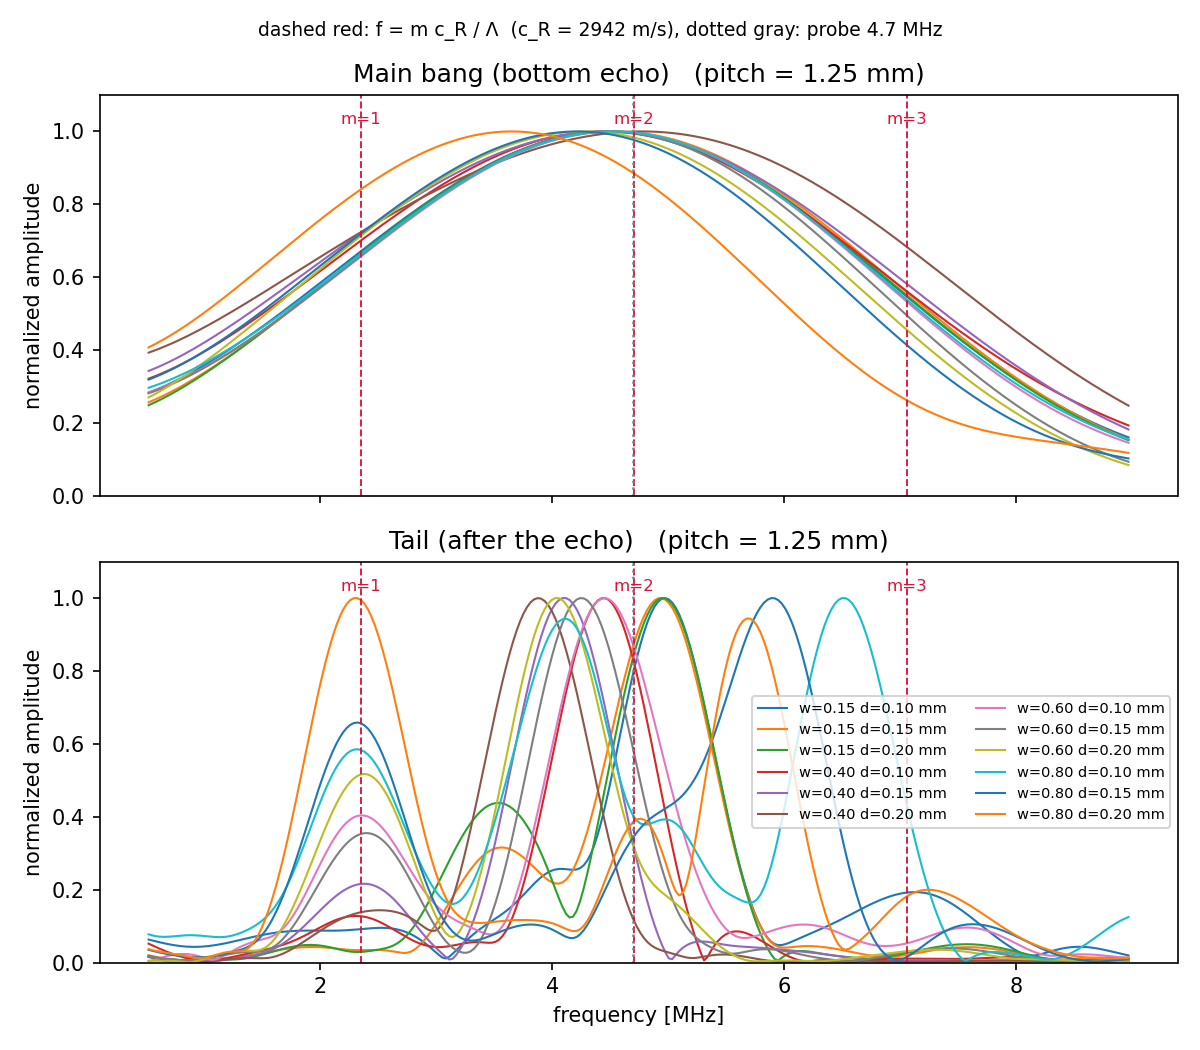
\includegraphics[width=8.0cm]{../../tmp_output/wood_anomaly/tail_spectrum_pitch125.png}
    \vspace{-2mm}
    \fgcaption{Main bang / tail spectra (pitch 1.25 mm)}
  \end{minipage}
  \hfill
  \begin{minipage}[b]{0.49\linewidth}
    \centering
    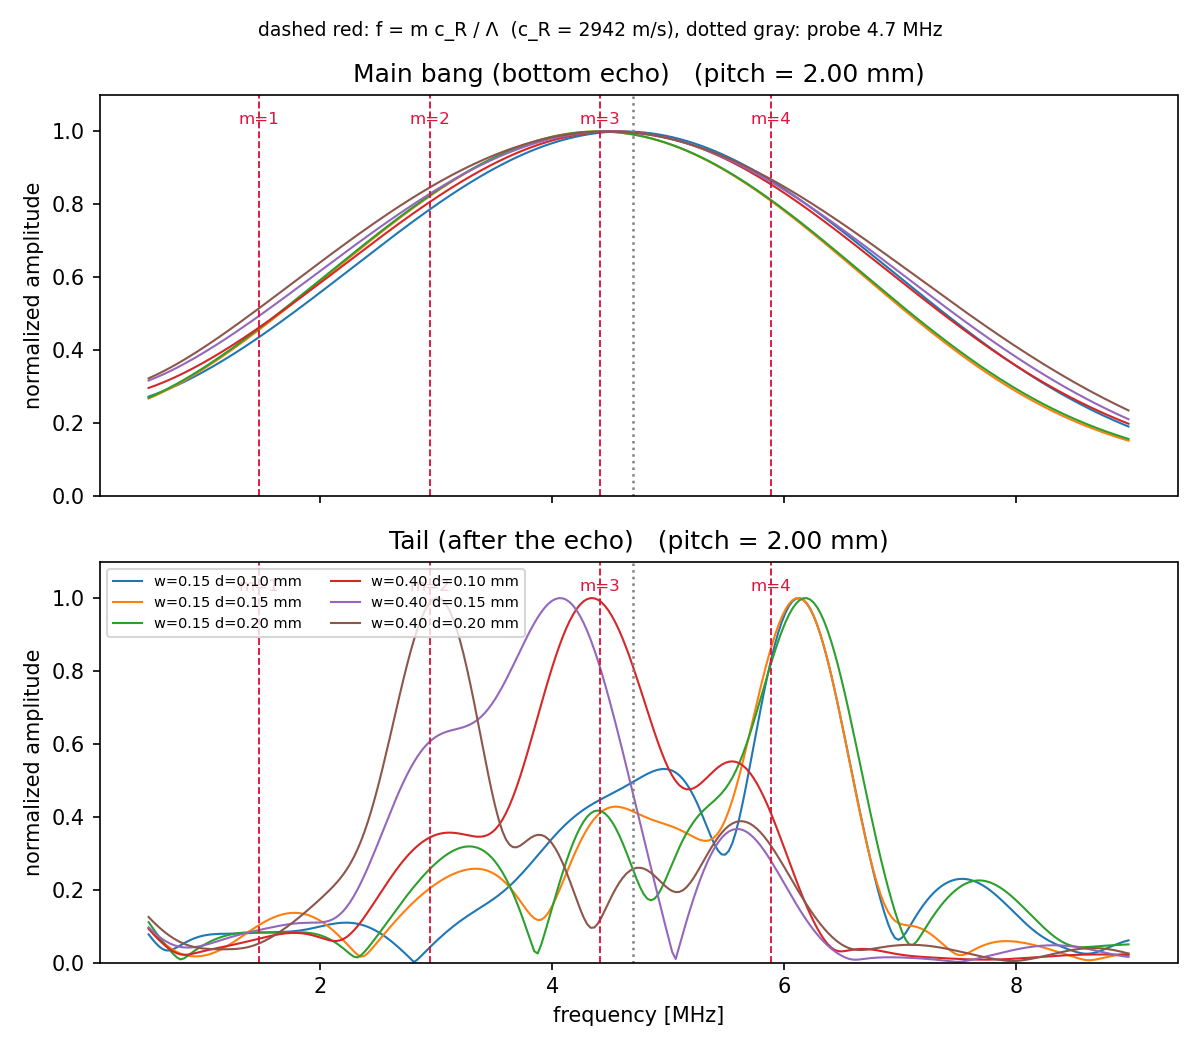
\includegraphics[width=8.0cm]{../../tmp_output/wood_anomaly/tail_spectrum_pitch200.png}
    \vspace{-2mm}
    \fgcaption{Main bang / tail spectra (pitch 2.00 mm)}
  \end{minipage}
  \label{fig:tail}
\end{center}

\par
図\ref{fig:tail} に示すように，メインバンのスペクトルは18条件全てにおいてほぼ同一であり，探触子固有の帯域特性をそのまま反映している．対照的に，テイルのスペクトルは溝の条件（ピッチ等）によって大きく変化している．これは，溝（傷）の幾何学的情報はメインバンではなくテイルに載っているという文献[1][2]の主張と整合する結果である．

\begin{center}
 \tbcaption{テイルとメインバンの振幅比（各条件の最大値の比，1--9\,MHz）}
 \vspace{1mm}
 \begin{tabular}{|c|c|r|r|r|} \hline
  \multirow{2}{*}{ピッチ [mm]} & \multirow{2}{*}{幅 [mm]}
   & \multicolumn{3}{c|}{深さ [mm]} \\ \cline{3-5}
   & & 0.10 & 0.15 & 0.20 \\ \hline\hline
  \multirow{4}{*}{1.25}
   & 0.15 & 0.105 & 0.182 & 0.271 \\
   & 0.40 & 0.211 & 0.405 & 1.415 \\
   & 0.60 & 0.101 & 0.382 & 0.697 \\
   & 0.80 & 0.055 & 0.208 & 0.364 \\ \hline
  \multirow{2}{*}{2.00}
   & 0.15 & 0.048 & 0.065 & 0.060 \\
   & 0.40 & 0.078 & 0.121 & 0.137 \\ \hline
 \end{tabular}
 \label{tab:ratio}
\end{center}

\par
さらに，表\ref{tab:ratio} に示す通り，テイルの最大振幅をメインバンの最大振幅で割った比（テイル／メインバン比）は，同一ピッチ・幅の群において溝の深さに対して単調増加する傾向が見られた（全6群中5群で成立）．唯一の例外であるピッチ 2.00 mm・幅 0.15 mm の群は，テイルの信号対雑音比（SNR）が約30と最も低く（他群は40〜210），ノイズの影響による逆転と考えうる．

\par
しかしながら，本解析には周波数分解能の制約という限界がある．テイルの窓長が $2.1\,\mathrm{\mu s}$ であるため，周波数分解能は 0.48 MHz に留まり，レイリー波の予測値（2.354 MHz）とS波の予測値（2.556 MHz）を明確に分離することができない．また，4.7 MHz 付近のピークも探触子の本来の帯域ピークと重なって区別が困難である．したがって，現段階の実験データから確実に言えるのは「テイル部にピッチに依存したスペクトル構造が存在する」という事実までである．


% =====================================================================
\section{本研究への含意と今後の方針}
% =====================================================================
\par
最終目標である PINN 等を用いた欠陥パラメータの逆推定に向け，本週の検討から以下の含意が得られた．

まず，回折格子方程式（式(\ref{eq:grating})）には凹凸のピッチ $\Lambda$ のみが含まれ，深さや幅は関与しない．すなわち，テイルスペクトルの異常周波数の位置からはピッチの情報しか抽出できない．
深さの情報を含む特徴量としては，次の2つの候補が考えられる．第一に，文献[2]（第3章）で議論されているサブハーモニック回折である．これは溝内部での多重反射に伴う追加の位相変化に起因し，深さに依存する．第二に，本研究の予備解析で確認された「テイル／メインバン振幅比」（表\ref{tab:ratio}）である．これは実データから直接観測された量であり，深さの単調関数となっている可能性が高いため，逆推定の特徴量として優先的に試行する価値がある．

また，文献[2]（第5章）では，凹凸形状を正確に評価するための距離分解能の条件として $R \le H$（$R = \tau c/2$，$\tau$ はパルス長）が示されているが，本研究の条件（深さ $H \le 0.20\,\mathrm{mm}$）ではこれを満たせない．飛行時間（TOF）の差で直接分離するには $\tau \le 0.070\,\mathrm{\mu s}$ が必要となるが，中心周波数 4.7 MHz の探触子では 0.33 波長分に過ぎず実現不可能である．これは文献[2]（8.3節）でも「今後の課題」として指摘されている困難なケースそのものであり，対策としてパルス超音波のコムフィルタ効果（位相シフト関係）の利用などが挙げられており，今後のモデル構築の参考となる．

\subsection{次に行うこと}
\begin{itemize}
 \item \textbf{平滑面（傷なし）の参照シミュレーションの実行}: 文献における解析は全て「凹凸面」と「平滑面」の比較に基づいており，テイル成分が傷由来か装置由来かを切り分けるために必須である．
 \item \textbf{シミュレーション波形を用いたテイル解析}: 帯域制限やノイズのない理想的な条件下で，予測された異常周波数が発現するかを，分解能の制約を排除して厳密に検証する．
 \item \textbf{ソノグラム（時間--周波数表示）の作成}: 単純な FFT では位相や時間遅れの判別が困難なため，エネルギーの遅延到達を視覚化し，物理機構を裏付ける．
 \item \textbf{窓処理の適用範囲の再確認}: 既存の波形切り出し処理（窓処理）が，情報を含むテイル部を意図せず切り落としていないかを確認し，適切に修正する．
\end{itemize}

%
\end{document}
